\documentclass[a4paper]{article}
\title{MA2: $\{ \sin (k) \mid k \in \mathbb{Z} \}$}
\author{Tommy Chu}
\date{}

\usepackage[czech]{babel}
\usepackage[utf8]{inputenc}
\usepackage[T1]{fontenc}
\usepackage{graphicx}
\usepackage{amsmath}
\usepackage{amsthm}
\usepackage{amssymb}
\usepackage{subfiles}
\usepackage{hyperref}
\usepackage{geometry}
\usepackage{mathtools}
\usepackage{algpseudocode}
\usepackage{algorithm}
\usepackage{physics}
\usepackage{dsfont}
\usepackage{bm}
\usepackage{bbm}
\usepackage{float}
\usepackage{enumitem}
\usepackage{graphicx}
\usepackage{multirow}
\usepackage{tikz}
\usepackage{tikz-cd}
\usepackage{pgfplots}
\usepackage{lmodern}
\usepackage{import}
\usepackage{microtype}
\usepackage{fancyhdr}
\usepackage{parskip}
\usepackage{titling}

\graphicspath{ {./images/} }

\microtypesetup{
    protrusion=true,
    activate={true,nocompatibility},
    final,
    tracking=true,
    kerning=true,
    spacing=true,
    factor=1100,
}

\relpenalty   = 10000
\binoppenalty = 10000

\setlength{\droptitle}{-5em}

\begin{document}
\maketitle

\section*{Zadání}

Dokažte, že množina $\{ \sin (k) \mid k \in \mathbb{Z} \}$ je hustá v $[-1, 1]$.

\subsection*{Pomocná tvrzení}

\subsubsection*{Tvrzení 1}

Nechť je $M$ podgrupa $(\mathbb{R}, +)$. Pro $M$ platí právě jedna z následujících vět:

$A$: Existuje kladné minimum $M$. \\
$B$: $M$ je hustá v $\mathbb{R}$.

\paragraph*{Důkaz:}
$(A \Rightarrow \neg B)$: Pokud má $M$ kladné minimum $m$, pak průnik intervalu $(\frac{m}{4}, \frac{m}{2})$ s~množinou $M$ je prázdný. $M$ tedy není v $\mathbb{R}$ hustá.

\begin{center}
    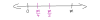
\includegraphics[height=1.6cm]{1a}
\end{center}

$(\neg A \Rightarrow B)$: Neexistuje-li kladné minimum $M$, pak pro libovoné $\varepsilon > 0$ existuje $m \in M$ takové, že $0 < m < \varepsilon$. Pro libovolné $x \in \mathbb{R}$ nutně existuje $k \in \mathbb{Z}$, pro~které platí $k m \leq x < (k + 1) m$. Po odečtení $km$ obdržíme ${0 \leq x - k m < m < \varepsilon}$, což lze přepsat na $|x - k m| < \varepsilon$, tedy pro libovolný interval $(x - \varepsilon, x + \varepsilon)$ existuje $km \in M$, který v něm leží. Množina $M$ je v $\mathbb{R}$ hustá.
\qed

\begin{center}
    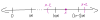
\includegraphics[height=1.6cm]{1b}
\end{center}

\subsubsection*{Tvrzení 2}

Uvažujme $M$ z předchozího tvrzení. Pokud $M$ není v $\mathbb{R}$ hustá, pak ${M = \{km \mid k \in \mathbb{Z}\}}$, kde $m$ je kladné minimum množiny $M$.

\paragraph*{Důkaz:}
Existenci kladného minima $m$ zajišťuje Tvrzení 1, $\{km \mid k \in \mathbb{Z}\} \subseteq M$ plyne z~uzavřenosti vůči sčítání. Pro spor předpokládejme, že existuje prvek ${r \in M \setminus \{km \mid k \in \mathbb{Z}\}}$. Pro tento prvek jistě existuje $k \in \mathbb{Z}$ takové, že $k m < r < (k + 1) m$. Po odečtení $km$ obdržíme $0 < r - k m < m$, kde $ r - k m \in M$. To je však ve sporu s tím, že $m$ je kladným minimem $M$.
\qed

\begin{center}
    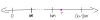
\includegraphics[height=1.6cm]{2}
\end{center}

\subsubsection*{Tvrzení 3}

Uvažujme $M = \{a + 2\pi b \mid a, b \in \mathbb{Z}\}$. $M$ je hustá v $\mathbb{R}$.

\paragraph*{Důkaz:}
Pro spor předpokládejme, že $M$ není v $\mathbb{R}$ hustá. Pak podle Tvrzení 1 existuje kladné minimum $m = a_m + 2\pi b_m \in M$, kde $a_m, b_m \in \mathbb{Z}$. Dále z Tvrzení~2 vyplývá, že $M = \{km \mid k \in \mathbb{Z}\}$. Z toho plyne
\[
    \mathbb{Z} = \{a \mid a \in \mathbb{Z}\}
    \subseteq \{a + 2\pi b \mid a, b \in \mathbb{Z}\}
    = M = \{km \mid k \in \mathbb{Z}\} \\
\]
\[
    1 \in \mathbb{Z}
    \implies 1 \in M
    \implies (\exists k \in \mathbb{Z})(1 = k m = k (a_m + 2\pi b_m))
\]
Z toho však plyne $\pi = \frac{1 - k a_m}{2k b_m} \in \mathbb{Q}$, což je ve sporu s tím, že $\pi$ je iracionální.

Proto je množina $\{a + 2\pi b \mid a, b \in \mathbb{Z}\}$ v $\mathbb{R}$ hustá.
\qed

\subsection*{Řešení}

Uvažujme libovolné $x \in [-1, 1]$, $\varepsilon > 0$. Chceme ukázat, že existuje $n \in \mathbb{Z}$ takové, že $|x - \sin(n)| < \varepsilon$. Protože $H_{\sin} = [-1, 1]$, existuje $\varphi_x \in \mathbb{R}$ takové, že $x = \sin(\varphi_x)$. Navíc funkce sinus je spojitá, proto platí
\[ \lim_{\varphi \to \varphi_x} \sin(\varphi) = \sin(\varphi_x) = x \]

Díky tomu, že je množina $M = \{a + 2\pi b \mid a, b \in \mathbb{Z}\}$ v $\mathbb{R}$ hustá, existuje posloupnost $(s_n)^{\infty}_{n = 1}$ prvků z $M \setminus \{\varphi_x\}$ taková, že
\[\lim_{n \to \infty} s_n = \varphi_x \]

Odtud z Heineho věty plyne, že pro limitu posloupnosti $(\sin(s_n))^{\infty}_{n = 1}$ platí
\[\lim_{n \to \infty} \sin(s_n) = x \]

Prvky posloupnosti $(s_n)^{\infty}_{n = 1}$ jsou tvaru $a_n + 2\pi b_n$, kde $a_n, b_n \in \mathbb{Z}$. Funkce sinus má ovšem periodu $2\pi$, tedy lze vypustit $2\pi b_n$:
\[
    x = \lim_{n \to \infty} \sin(s_n)
    = \lim_{n \to \infty} \sin(a_n + 2\pi b_n)
    = \lim_{n \to \infty} \sin(a_n)
\]
Z toho vyplývá, že pro libovolně zvolené $\varepsilon > 0$ existuje  $n \in \mathbb{Z}$ takové, že ${|x - \sin(n)| < \varepsilon}$.
\qed

\begin{center}
    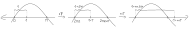
\includegraphics[height=5.6cm]{4}
\end{center}

\end{document}
